\mode<presentation>
{
  \usetheme{default} % no fancy navigation or anything ... 
  \usecolortheme{tobi}
  \usefonttheme{serif}   
  \usepackage{lmodern}
  \newcommand{\addgraph}[1]{\includegraphics[width=\textwidth]{ex/#1}}
  \setbeamercovered{transparent=100}
\AtBeginSection[]
{
   \begin{frame}
     \begin{center}
     \Large\textbf{\insertsection}
   \end{center}
   % \frametitle{Outline}
%      \tableofcontents[currentsection]
   \end{frame}
}
}
\mode<article>
{
  \usepackage{url}
  \usepackage{graphicx}
  \usepackage[colorlinks,hyperindex,plainpages=false]{hyperref}
  \setlength{\parskip}{1ex plus 0.5ex minus 0.2ex}
  \setlength{\parindent}{0pt}  
  \usepackage{times}
  \newcommand{\addgraph}[1]{\begin{center}\framebox{\includegraphics[width=0.9\textwidth]{ex/#1}}\end{center}}
  \addtolength{\voffset}{-2.5cm}
  \addtolength{\textheight}{4cm}
}
\usepackage{alltt}
\usepackage{listings}
\usepackage{svgcolor}
\usepackage[english]{babel}
\usepackage[latin1]{inputenc}
% or whatever

\usepackage[T1]{fontenc}
% Or whatever. Note that the encoding and the font should match. If T1
% does not look nice, try deleting the line with the fontenc.

\title
{RRDtool advanced Topics}

\author
{Tobias Oetiker}

\institute
{OETIKER+PARTNER AG}

\date[LISA 2011] % (optional, should be abbreviation of conference name)
{25th Large Installation System Administration Conference}

\mode<presentation>{\subject{RRDtool tutorial based on example use}}

\mode<presentation>{
 \lstset{%
   language=Perl,%
   numbers=left,%
   basicstyle=\ttfamily\footnotesize\color{black},%
   keywordstyle=\color{darkgreen},%
%  identifyerstyle=\color{brown},%
   commentstyle=\color{mediumpurple},%
   stringstyle=\color{dimgray},
   numberstyle=\ttfamily\scriptsize\color{darkgray},
   showstringspaces=false
 }
}
\mode<article>{
 \lstset{%
   language=Perl,%
   numbers=left,%
   basicstyle=\ttfamily\footnotesize,%
   keywordstyle=\bfseries,%
   numberstyle=\ttfamily\scriptsize,
%  identifyerstyle=\color{brown},%
   commentstyle=\itshape,%
   stringstyle=\color{black},
   showstringspaces=false
 }
}

\begin{document}

\mode<article>{\maketitle}

\begin{frame}<presentation>
  \titlepage
\end{frame}

\mode<articel>{\tableofcontents}

\section{A different kind of Database}

\begin{frame}{creating a simple rrd}
\lstinputlisting[language=bash,firstline=0,lastline=11]{ex/create-first.sh}
One Datasource, 4 Round Robin Archives
\end{frame}

\begin{frame}{feeding data}
\lstinputlisting[language=bash,firstline=13,lastline=21]{ex/create-first.sh}
Feed in some data. One or several updates at once.
\end{frame}

\begin{frame}[allowframebreaks]{inside the database}
\lstinputlisting[language=xml,basicstyle=\ttfamily\scriptsize]{ex/create-first.xml}
\end{frame}

\mode<article>{
The xml dump of the rrd file shows an approximation of the on-disk
structure of the database. The rra database sections are re-ordered, so that
they are in chronological order with the oldest at the top. Also the
cdp sections are stored right after the header. The idea behind this
design is that data that get written on every update is as close
together as possible.}

\begin{frame}{rrd features}
\begin{itemize}[<+-| alert@+>]
\item optimized for time-series data
\item fixed size rotating data store
\item constant on-disk size
\item no maintenance
\item on the fly consolidation
\end{itemize}
\end{frame}

\begin{frame}[fragile]{on-disk structure}
\begin{alltt}
+-------------------------------+
| Static Header                 | \textrm{RRD cookie, DB cfg}
|-------------------------------|\pause 
: Data Source (DS) Definitions  : 
|-------------------------------|\pause
: RR Archive (RRA) Definitions  : 
|===============================|\pause
| Live Head                     | \textrm{last update time}
|-------------------------------|\pause 
: PDP Prep per DS               : \textrm{last value for diff}
|-------------------------------|\pause
: CDP Prep per RRA and DS       : \textrm{intermediate storage}
|-------------------------------|\pause
: RRA Pointers                  :
|===============================|\pause
: Round Robin Archives (RRA)    :
+-------------------------------+
\end{alltt}
\end{frame}

\begin{frame}{irregular data arrival intervals}
\lstinputlisting[language=bash,lastline=19]{ex/update-real.sh}
\end{frame}

\mode<article>{To try things out lets assume that data arrives at
  irregular intervals. This is counter data. By synchronizing the
  data values with the arrival time we should get a constant rate
  stored in the database.}

\begin{frame}{database after the irregular updates}
\lstinputlisting[language=bash,firstline=20]{ex/update-real.sh}
\lstinputlisting[language=bash]{ex/update-real.txt}

\begin{itemize}[<+-| alert@+>]
\item rrdtool re-binning at work
\item major difference to a normal db
\item all bins contain 1.0
\item the time is the 'end-time' of the bin.
\end{itemize}
\end{frame}

\begin{frame}{optimizing your rrds}
\begin{itemize}[<+-| alert@+>]
\item update of multi DS RRD is cheep
\item single update interval per RRD
\item RRD modification is expensive
\item RRD size and update performance are independent
\item RRA complexity affects update performance
\end{itemize}
\end{frame}

\mode<article>{As long as your system is small (a few hundred RRDs)
  you should optimize for convenience. Only keep DSes together
  in one RRD that are tightly bound. For everything else
  create separate RRDs.}

\begin{frame}{fetching data}
fetch is for reading data from an rrd
\lstinputlisting[language=bash,firstline=8,lastline=9]{ex/catch-fetch.sh}
\begin{itemize}[<+-| alert@+>]
\item one RRA with two 300s entries
\item one RRA with three 600s entries
\end{itemize}
\end{frame}

\begin{frame}[fragile]{playing catch with fetch}
first pull 300 seconds
\begin{verbatim}
> rrdtool fetch x.rrd -r 300 \
  -s 1200000600 -e 1200000900 AVERAGE

1200000900: 4.0000000000e+01
1200001200: 5.0000000000e+01
\end{verbatim}

then pull 900 seconds
\begin{verbatim}
> rrdtool fetch x.rrd -r300 \
  -s 1200000000 -e 1200000900 AVERAGE

1200000600: 2.5000000000e+01
1200001200: 4.5000000000e+01
\end{verbatim}
\end{frame}

\begin{frame}{fetch recap}
\begin{itemize}[<+-| alert@+>]
\item looking for complete coverage
\item resolution is only a suggestion
\item time stamp in output marks the END of the period
\item end-time differences caused problems
\item since 1.3, only the start-time is relevant for coverage
\item outside the rra everything is NaN
\end{itemize}
\end{frame}

\mode<article>{\newpage}

\section{Graphing}
\begin{frame}[fragile]{rrdgraph syntax 101}
for graph command syntax, there are two basic rules:\pause
\begin{enumerate}
\item \texttt{-{}-options} start with a double dash\pause
\item graphing instructions start with a letter
\end{enumerate}

\pause
\begin{center}
\renewcommand{\tabcolsep}{0.4cm}
\renewcommand{\arraystretch}{2}

\begin{tabular}{|l|}\hline
\begin{minipage}[t]{0.7\textwidth}
\begin{alltt}
rrdtool graph \textit{output}
   DEF:var=\textit{rrd}:\textit{DS}:\textit{AVARAGE}
   LINE:var#\textit{hex-rgb-color}:Comment

\end{alltt}
\end{minipage}\\\hline
\end{tabular}
\end{center}

\texttt{DEF} and \texttt{LINE} are \emph{graphing instructions}.
\end{frame}

\mode<article>{The rrd graph command is the most versatile of all rrdtool
  commands. It comes with its own little language, optimized for
  drawing graphs. There are two kinds of arguments. The options
  which start with a double-dash and the graphing instructions that
  start with an uppercase letter.}

\begin{frame}{normal line}
\addgraph{LINE}
\end{frame}

\begin{frame}{lower limit}
\addgraph{LINE-lower}
\end{frame}

\mode<article>{Unless you are a banker and are you drawing stock diagrams,
  make sure your graph displays the zero-y-value. Otherwise it is
  pretty difficult to judge the meaning of the graph since perspective
  is limited to the numbers on the y-axis.}

\begin{frame}{slope mode}
\addgraph{LINE-slope}
\end{frame}

\mode<article>{RRD graphs are pretty blocky. This is on purpose, since
  the data is blocky too. The slope mode is a little concession. It
  tilts the vertical connections between the 'blocks' by one pixel.}

\begin{frame}{anti-anti-aliasing: graph}
\addgraph{LINE-graph-mono}
\end{frame}

\begin{frame}{anti-anti-aliasing: font}
\addgraph{LINE-font-mono}
\end{frame}

\mode<article>{\newpage}
\begin{frame}{line width}
\addgraph{LINE-width}
\end{frame}

\begin{frame}{dashed line}
\addgraph{LINE-dash}
\end{frame}

\mode<article>{The numbers are an ON-OFF-ON-OFF-\ldots pattern. The
  \texttt{dash-offset} property lets you shift the dashing of the line
  to the right.}

\mode<article>{\newpage}

\begin{frame}{DEF with :step}
\addgraph{DEF-step}
\end{frame}


\begin{frame}{DEF with :start}
\addgraph{DEF-start}
\end{frame}
\mode<article>{\newpage}

\begin{frame}{DEF with :reduce}
\addgraph{DEF-reduce}
\end{frame}

\begin{frame}{AREA simple}
\addgraph{AREA-simple}
\end{frame}

\mode<article>{\newpage}
\begin{frame}{two AREAs}
\addgraph{AREA-two}
\end{frame}

\begin{frame}{transparent AREA}
\addgraph{AREA-trans}
\end{frame}

\mode<article>{RRDtool creates real alpha transparency. You can set
  the whole graph to be transparent by setting the 
  graph CANVAS and BACKGROUND colors to transparent.}

\mode<article>{\newpage}
\begin{frame}{stacked AREA}
\addgraph{AREA-stack}
\end{frame}

\mode<article>{\newpage}

\begin{frame}{time shift}
\addgraph{SHIFT-simple}
\end{frame}

\begin{frame}{shifting with extra data}
\addgraph{SHIFT-startdef}
\end{frame}

\mode<article>{A normal \texttt{DEF} line requests exactly as much data as it
requires for drawing the graph. If you \texttt{SHIFT} the data, you
may want to adjust the data fetched accordingly.}

\mode<article>{\newpage}
\section{Revers Polish Notation (RPN) Math}

\mode<article>{RRDtool lets you apply math operations to the data
  prior to showing it to the user. It uses RPN math for this. If you
  ever owned a classic HP calculator, you may still remember how RPN
  math works. For all the others there is a little example below,
  that shows how to do a little addition in RPN.}

\begin{frame}[fragile]{RPN basics: Step 0}
$15+23=38$
\begin{alltt}
            1: NAN
            2: NAN
            3: NAN
\end{alltt}
\end{frame}
\begin{frame}[fragile]{RPN basics: Step 1}
$\mathbf{15}+23=38$
\begin{alltt}
[15]        1: \textbf{15}
            2: NAN
            3: NAN
\end{alltt}
\end{frame}
\begin{frame}[fragile]{RPN basics: Step 2}
$15+\mathbf{23}=38$
\begin{alltt}
[23]        1: \textbf{23}
            2: 15
            3: NAN
\end{alltt}
\end{frame}
\begin{frame}[fragile]{RPN basics: Step 3}
$15\mathbf{+}23=38$
\begin{alltt}
[+]         1: \textbf{38}
            2: NAN
            3: NAN
\end{alltt}
\end{frame}

\newpage 

\begin{frame}{math in the graph (+)}
\addgraph{RPN-simple}
\end{frame}

\mode<article>{A simple addition. We add a fixed value to a data
  source. Note that at least one data source must appear inside a CDEF
  expression. The input to a CDEF expression can come from another
  CDEF expression.}

\begin{frame}{simple gradient}
\addgraph{RPN-grad-a}
\end{frame}

\begin{frame}{the MAX function}
\addgraph{RPN-max}
\end{frame}

\mode<article>{The MAX function operates on two values. In this example
  the input comes from two different data sources.}

\begin{frame}{the LIMIT function}
\addgraph{RPN-limit}
\end{frame}

\mode<article>{The \texttt{LIMIT} function will return UNKNOWN as soon
  as the input value is outside the given range. UNKNOWN data does not
  get drawn.}

\begin{frame}{the TREND function}
\addgraph{RPN-trend}
\end{frame}

\mode<article>{If a data source varies massively, the TREND function
  lets you smooth away by building a moving average. By calculating
  the average, the output gets shifted by the length of the TREND
  calculation.}

\begin{frame}{the TREND with early start}
\addgraph{RPN-trend-start}
\end{frame}

\mode<article>{In the previous graph there was a bit of data missing
  at the left border of the graph. This was because rrdgraph loads
  exactly the amount of data that is required in the graph (yes same
  story as before). By loading more data, we can provide the TREND
  function with enough input, so that it can calculate the first few
  pixels as well.}

\begin{frame}{the TREND and SHIFT}
\addgraph{RPN-trend-shift}
\end{frame}

\mode<article>{Another interesting option is to SHIFT the result of
  the TREND calculation back in time, so that it matches with the
  source data. This allows us to see more easily when there are
  'outliners'}

\mode<article>{\newpage}


\begin{frame}{the IF function}
\addgraph{RPN-if}
\end{frame}

\mode<article>{The IF function requires three items on the stack. It
  turns \texttt{a,b,c,IF} into \texttt{if a then b else c}. There is a
  bunch  of operators that go along with the \texttt{IF}: \texttt{LT}
  less, \texttt{LE} - less or equal, \texttt{EQ} - equal, \texttt{NE}
  not equal, \texttt{GE} - greater or equal, \texttt{GT} - greater.}

\begin{frame}{horizontal gradient}
\addgraph{RPN-grad-b}
\end{frame}


\begin{frame}{about invisibility}
\addgraph{RPN-UNKN}
\end{frame}

\mode<article>{Unknown values are not drawn on the graph. Here we
  use trick to only show the largest values.}


\begin{frame}{positional drawing count}
\addgraph{RPN-count}
\end{frame}

\mode<article>{If you are into bar charts, you might fake them with
  this trick. COUNT, counts the values of the data set. We use this,
  together with the modulo operator to suppress the drawing of every
  third entry.}

\begin{frame}{access the previous value}
\addgraph{RPN-prev}
\end{frame}

\begin{frame}{positional drawing time}
\addgraph{RPN-time}
\end{frame}

\newpage
\begin{frame}{positional drawing time-shifting}
\addgraph{RPN-time-minus}
\end{frame}

\mode<article>{There is also a function for accessing the Unix time
  (seconds since 1970) associated with the graph data. With it, you
  can make your stripes a fixed number of seconds wide.}

\begin{frame}{time and resolution issues}
\addgraph{RPN-time-odd}
\end{frame}

\mode<article>{\newpage}

\mode<article>{Whenever RRDtool graph has to do math with data sets
  that come in different step sizes, it first to adjust the step sizes
  so that they match. To do this, it finds the greatest common divisor
  and uses it as the new step size.}

\begin{frame}[fragile]{CDEF internals}
\begin{itemize}[<+-| alert@+>]
\item data may come in different resolutions
\item all items in a CDEF must have the same resolution
\item resolution is expanded to greatest common devisor (gcd)
\item example: gcd(6,9) = 3, gcd(1,6) = 1
\end{itemize}

trick: an rrd with one a second step.
\begin{alltt}
rrdtool create one.rrd --step=1
   DS:one:GAUGE:2:U:U
   RRA:AVERAGE:0.5:1:1
\end{alltt}
\end{frame}

\begin{frame}{step=1 trick: high resolution cdef}
\addgraph{RPN-time-odd-hires}
\end{frame}

\mode<article>{By introducing this special rrd with a ``one second
  step'' the greatest common divisor (gcd) becomes one.}

\section{Consolidation functions}

\begin{frame}{finding the average}
\addgraph{VDEF-average}
\end{frame}

\begin{frame}{calculating min and max}
\addgraph{VDEF-minmax}
\end{frame}


\mode<article>{\newpage}

\begin{frame}[fragile]{min max code example}
\begin{alltt}
LINE:a#456:a
VDEF:max=a,MAXIMUM
LINE:max#123
VRULE:max#123:maximum
GPRINT:max:%.1lf
GPRINT:max:%H\(\backslash\):%M\textbf{:strftime}
\end{alltt}
A VDEF result has a value and a time assigned.
\end{frame}

\begin{frame}{Least Squares Line (y=x*m+b)}
\addgraph{VDEF-lsl}
\end{frame}

\mode<article>{\newpage}
\section{Holt Winters Aberrant Behaviour Detection}

\begin{frame}{about alert generation}
\begin{itemize}[<+-| alert@+>]
\item when something unexpected happens send an alert
\item fixed thresholds are too wide a net
\item moving averages weigh all data equal
\item holt winters can predict the future
\item and no one considers himself clever enough to use it
\end{itemize}
\end{frame}

\begin{frame}{rrd - holt winters assumptions}
\begin{itemize}[<+-| alert@+>]
\item data is periodic in nature
\item data has continuity 
\item data continuity is periodic
\item recent data is more important
\end{itemize}
\end{frame}

\begin{frame}{holt winters aberrant behavior}
\begin{itemize}[<+-| alert@+>]
\item prediction of future value and confidence band
\item confidence band is like a standard deviation
\item real value compared to predicted value +/- confidence band
\end{itemize}
\end{frame}

\mode<article>{With holt winters RRDtool will calculate a prediction
  and a confidence band (think of it as a standard deviation) for the
  current value. It will then compare the prediction with the
  actual value. If the actual value falls outside the confidence band
  of the predicted value (or some multiple of it), then a confidence
  band violation is registered. If multiple violations are registered
  within a configurable interval, RRDtool logs a failure.}

\begin{frame}<presentation>{holt winters configuration}
\begin{itemize}[<+-| alert@+>]
\item HWPREDICT for starters
\item tweaking required
\item know the knobs to turn
\item use real data to test
\item FAILURES very short
\item \texttt{rrdtool tune} and \texttt{resize}
\end{itemize}
\end{frame}

\mode<article>{
\begin{itemize}[<+-| alert@+>]
\item Keep it simple, go for HWPREDICT only when you start using
  holt winters in RRDtool.
\item Every data set is different, tweaking is required. 
\item Know which knobs to turn.
\item Use real data when experimenting.
\item Use \texttt{rrdtool tune} and \texttt{rrdtool resize} to tweak settings.
\item The FAILURES RRA is short!
\end{itemize}
}

\begin{frame}{holt winters parameters}
\texttt{RRA:HWPREDICT:}\emph{rows}\texttt{:}\emph{alpha}\texttt{:}\emph{beta}\texttt{:}\emph{period}

\begin{description}
\item[\emph{alpha}:] adaption rate of the baseline (1 fast, 0 slow)
\item[\emph{beta}:] adaption rate of the slope (1 fast, 0 slow)
\item[\emph{period}:] how many steps in a period (use 1 to  disable)
\item[\emph{gamma}:] seasonal adaption rate of the baseline\\(alpha by
  default)
\item[\emph{dev\_gamma}:] seasonal adaption rate of the confidence
  band\\
 (gamma by default)
\end{description}

the gamma and confidence band are tunable with \texttt{rrdtool tune}
\end{frame}

\mode<article>{
Reading \href{http://cricket.sourceforge.net/aberrant/lisa2000_paper.pdf}{Brutlag's original paper}
I wrote down the formulas he uses for calculating holt winters. This
helped me quite a lot in understanding the relationships between
alpha, beta, gamma and delta.}

\begin{frame}[fragile]{the rrdtool holt winters formula}
\begin{small}
\begin{alltt}
a - baseline (RRA CDP Parameter)
b - slope (RRA CDP Parameter)
c - seasonal (SEASONAL RRA)
d - deviation (DEVSEASONAL RRA)
pred - predicted value
real - real value\pause

pred\{next\} = a\{now\} + b\{now\} + c\{next_prev_period\}\pause

a\{now\} = alpha * (real\{now\} - c\{now_prev_period\}) 
         + (1-alpha) * ( a\{prev\} + b\{prev\})\pause
b\{now\} = beta  * (a\{now\} - a\{prev\}) 
         + (1-beta) * b_prev\pause
c\{now\} = gamma * (real\{now\} - a\{now\}) 
         + (1-gamma) * c\{now_prev_period\}\pause
d\{now\} = dev_gamma * abs(real\{now\} - pred\{now\}) 
         + (1-dev_gamma) * d\{now_prev_period\}\pause

\end{alltt}
\end{small}
\end{frame}

% must be formatted like that
% to break gobbling mode!
%\mode
%<all>

\begin{frame}{hw demo: the test data}
\addgraph{HW-input}

traffic at a peering point
\end{frame}

\begin{frame}[fragile]{drawing a hw graph}
\begin{lstlisting}[language=xml]
DEF:in=hw.rrd:in:AVERAGE
DEF:pred=hw.rrd:in:HWPREDICT
DEF:conf=hw.rrd:in:DEVPREDICT
DEF:fail=hw.rrd:in:FAILURES
TICK:fail#ff8:1:Failures
CDEF:lowconf=pred,conf,2,*,-
LINE1:lowconf
CDEF:confwidth=conf,4,*
AREA:confwidth#cfc:Band:STACK
LINE0.1:0#3a1::STACK
LINE0.1:lowconf#3a1
LINE1:in#c00:InOctets
LINE1:pred#0a0:Prediction
\end{lstlisting}
\end{frame}  

\mode<article>{For starters we set the period to 1. This disables HW's
  ability to adjust to periodic behavior in the data but it lets us
  better observe the effects of the different parameter settings since
  the adjustment period is much shorter.}

\begin{frame}{hw demo: alpha}
\addgraph{HW-p1-a0_5-b0_001}\\
\addgraph{HW-p1-a0_1-b0_001}
\end{frame}

\mode<article>{The smaller the alpha the slower the adaption. As the
  prediction is now generally off by quite a bit, this causes the
  confidence band to grow as well.}

\mode<article>{\newpage}

\begin{frame}{hw demo: beta}
\addgraph{HW-p1-a0_1-b0_001}\\
\addgraph{HW-p1-a0_1-b0_1}
\end{frame}

\mode<article>{The larger the beta the `heavier' the prediction
  becomes.}

\begin{frame}{hw demo: period}
\addgraph{HW-p1-a0_5-b0_001}\\
\addgraph{HW-p48-a0_5-b0_001}
\end{frame}

\begin{frame}{hw demo: tuning}
\addgraph{HW-p48-a0_5-b0_001}\\
\addgraph{HW-p48-a0_2-b0_001}
\end{frame}

\begin{frame}{hw demo: tuning II}
\addgraph{HW-p48-a0_2-b0_001}\\
\addgraph{HW-p48-a0_03-b0_001}
\end{frame}

\begin{frame}{hw demo: tuning III}
\addgraph{HW-p48-a0_03-b0_001}\\
\addgraph{HW-p48-a0_03-b0_1}
\end{frame}

\newpage

\section{The *v Interfaces}

\begin{frame}{graphv script}
\lstinputlisting{ex/v-interfaces.pl}
\end{frame}

\begin{frame}{graphv output}
\lstinputlisting{ex/v-interfaces.txt}
\end{frame}

\mode<article>{The image key only shows up when the graph file name is '-'.}

\begin{frame}{v-interfaces}
\begin{itemize}[<+-| alert@+>]
\item rrdtool info
\item rrdtool update\textbf{v}
\item rrdtool graph\textbf{v}
\end{itemize}
\end{frame}

\mode<article>{Using the output of updatev is much more efficient than
re-reading the rrd file after running normal update against them.}

\section{RRD Caching Daemon}

\begin{frame}{rrdcached --- pushing rrd performance}
\begin{itemize}[<+-| alert@+>]
\item i/o comes in 4k chunks
\item normal update is $\sim{}100$ bytes
\item grouping updates = performance for free
\item data in memory
\item journaling disaster recovery
\item simple integration using enviroment variables
\item communication via unix socket or ip
\item limited security for remote operation
\item no updatev support yet
\item available with 1.4
\end{itemize}
created by Florian Forster and Kevin Brintnall
\end{frame}

\section{Future}

\begin{frame}{Future RRDtool Features}
\begin{itemize}[<+-| alert@+>]
\item full remote support for rrdtool operations
\item getopt to popt migration for thread-safety
\item portable data format
\item in-memory updates for cached to support updatev
\item rrd internal journal for i/o optimization
\item separation of database and charting features
\item json interface and javascript charting frontend
\end{itemize}

\pause
Or anything else someone is willing\\
to provide time or money for.
\end{frame}


\section{Examples}

\begin{frame}{The size of an rrd - code}
\lstinputlisting{ex/rrd-size.pl}
\end{frame}

\begin{frame}{the size of an rrd - result}
\lstinputlisting{ex/rrd-size.txt}
\begin{itemize}[<+-| alert@+>]
\item overhead is minimal
\item 8 byte per double 
\item \ldots per datasource
\item \ldots per RRA
\item \ldots per RRA row
\end{itemize}
\end{frame}

\mode<article>{The rrd format is highly efficient at storing non
  sparse data. The overhead for an extra RRA or DS is normally a few
  bytes on top of the 8 byte per double.}


\newpage  
\section{Real Live Example}

\mode<article>{The following example shows how to create a simple
  traffic grapher with a shell script for data acquisition, and an
  rrdcgi script to draw the graphs.}

\begin{frame}
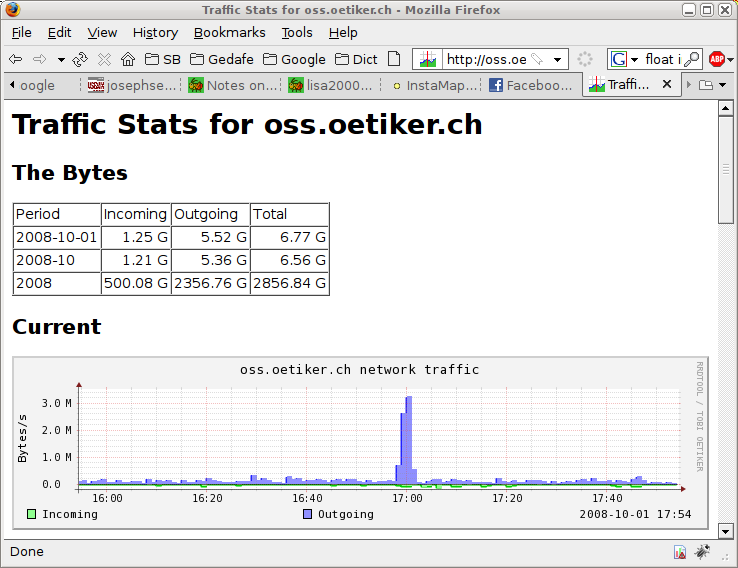
\includegraphics[width=\textwidth]{traffic/codewalk}
\end{frame}

\begin{frame}[allowframebreaks]{data acquisition}
\lstinputlisting[language=bash]{traffic/ifbyteget.sh}
\end{frame}

\mode<article>{This little bash script polls the network traffic
  counter from the linux proc tree and reformats it so that it can be
  fed to rrdtool.}

\begin{frame}[allowframebreaks]{rrdcgi: scripting for the poor}
\lstinputlisting[language=xml]{traffic/index.cgi}
\end{frame}

\begin{frame}[allowframebreaks]{rrdcgi: include file function}
\lstinputlisting[language=xml]{traffic/graph.inc}
\end{frame}

\mode<article>{RRDtool's rrdcgi is a very simple scripting engine, that can pick
  up pseudo xml elements from an html file and execute the
  coresponding rrdtool commands. In this example we use environment
  variables and an include file to save us from typing in the same
  graph definition over and over again.}

\mode<presentation>{
\begin{frame}
\begin{center}
\Huge ?
\end{center}
\end{frame}
\begin{frame}
\begin{center}
Tobi Oetiker <tobi@oetiker.ch>
\end{center}
\end{frame}
}

\mode<article>{
\vspace{\stretch{1}}
Tobias Oetiker <tobi@oetiker.ch>
}
\end{document}
%%% Local Variables:
%%% TeX-master: "presentation.tex"
%%% mode: flyspell
%%% TeX-PDF-mode: t
%%% End:
